\chapter{Planificación}

En este capítulo se describe la metodología utilizada en el proyecto, cómo se van a gestionar las tareas a lo largo del tiempo con un diagrama de Gantt y tras esto la evaluación del coste de todo el material y trabajo a realizar.

Por último se planteará otro diagrama de Gantt donde se muestran las franjas de las actividades de cómo han ocurrido de manera real y si son próximas a las estimadas.

\section{Metodología utilizada}

Respecto a la metodología utilizada va a ser una variante de Scrum, ya que se iran  realizando tareas (sprints) que serán evaluadas en periodos semanales por el tutor. Estas tienen el objetivo de ir expandiendo el producto poco a poco, y se puedan visualizar los diferentes requisitos aplicados. 

Tras la finalización de cada tareas, hay una reunión donde se discute la tarea realizada, y en el caso de cómo ha ido su desarrollo, se volverá a revisar o se avanzará a la siguiente tarea, pudiendo ir modificando la orientación del proyecto.

Además se ha hecho uso de un repositorio Github para realizar un control del siguiente proyecto. El link es el siguiente: \href{https://github.com/pparrilla/ROS2_TFG}{github.com/pparrilla/ROS2\_TFG}

\section{Temporización}

Para el registro de horas se va a utilizar la aplicación Clockify \cite{clockify}. Esta permite ir creando tareas diarias con un nombre, un tag referente a que grupo pertenece e indicar el proyecto. Este registro de horas es necesario para ir realizando comparaciones con el tiempo que se ha estimado para cada tarea.

A fecha de la planificación del proyecto se estima que con las horas llevadas a cabo, este durará unas 350-400h aproximadamente, dependiendo de si se han estimado bien el tiempo dedicado a cada tarea.

Por destacar, indicar que la temática llevaba establecida desde Abril de 2021, pero debido a que no se pudo empezar por cuestiones académicas, se ha acabado trasladando a estas fechas.

En el siguiente diagrama de Gantt \ref{fig:gantt} se detallan las diferentes tareas a realizar:

\begin{center}
    \centering
    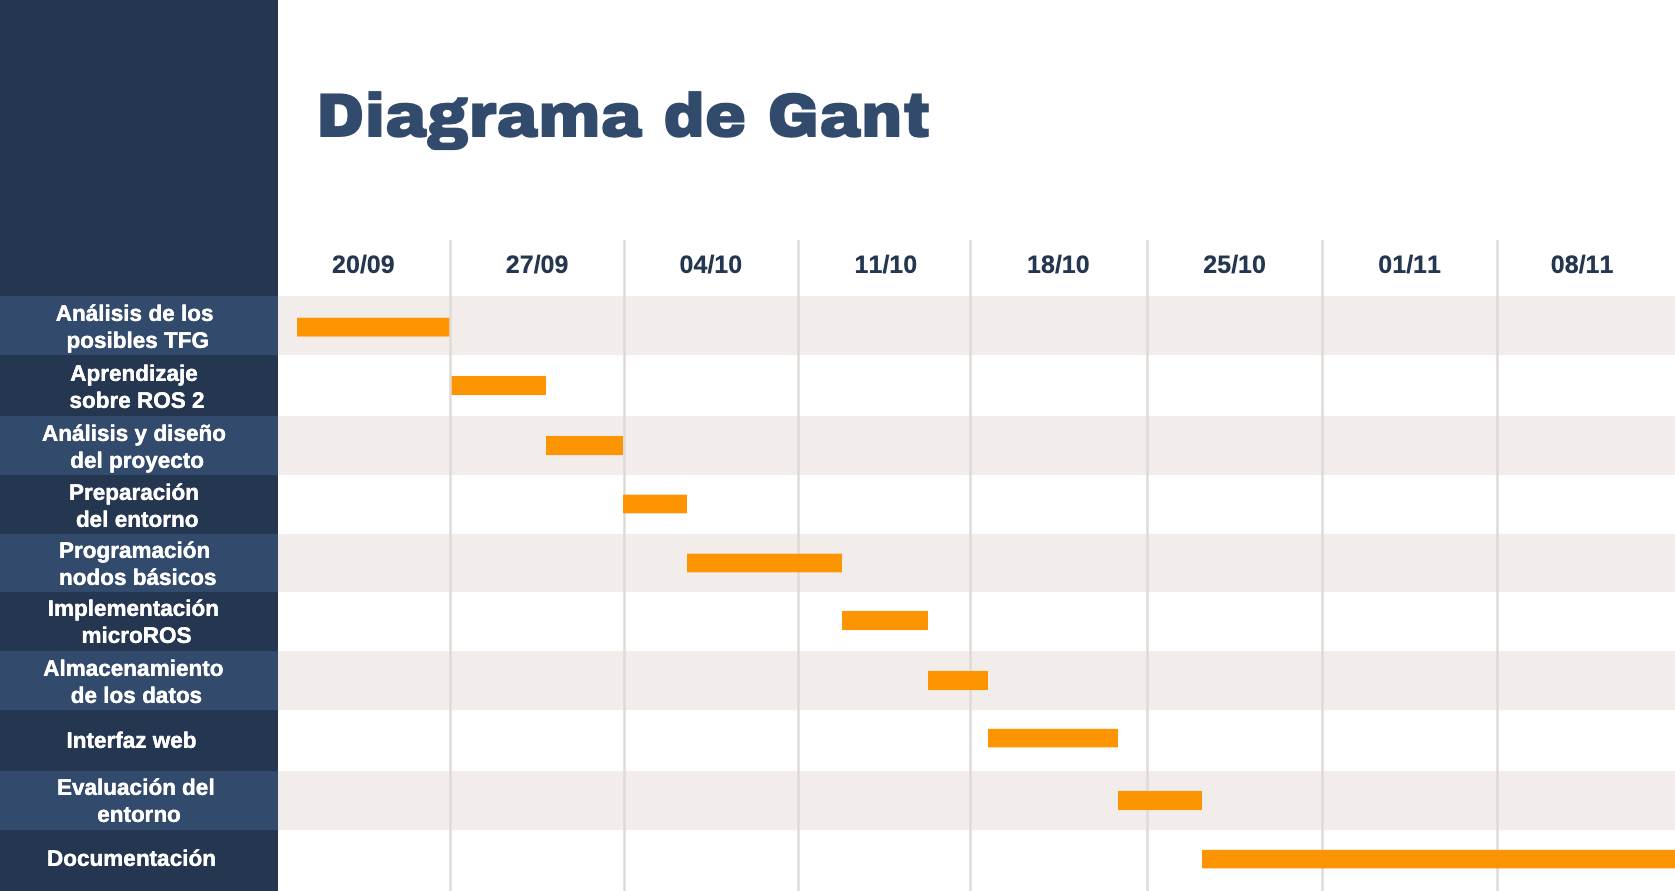
\includegraphics[width=\textwidth]{img/04-PreDiagrama-Gantt.png}
    \captionof{figure}{Diagrama de Gantt previo}
    \label{fig:pre-gantt}
\end{center}

Se van a explicar las diferentes categorías mostradas en el diagrama y que actividades abarcan cada una:

\begin{itemize}
    \item \textbf{Análisis de los posibles TFG.} Engloba la parte previa a la realización del proyecto, búsqueda de diferentes temáticas, información sobre las tecnologías a utilizar y casos de uso reales sobre este.
    \item \textbf{Aprendizaje sobre ROS 2.} Se agrupa el tiempo de aprendizaje de la tecnología y los conceptos relacionados.
    \item \textbf{Análisis y diseño del proyecto.} Una vez escogida la base del proyecto se establece la estructura del proyecto, elementos necesarios para su desarrollo tanto hardware y software, reestructuración de diferentes partes implementadas y derivados.
    \item \textbf{Preparación del entorno.} En los dispositivos utilizados es necesario la instalación y creación de un entorno de trabajo.
    \item \textbf{Programación nodos básicos.} Hace referencia a las implementaciones realizadas para los nodos principales a utilizar más el testeo de su funcionamiento.
    \item \textbf{Implementación microROS.} Para los microcontroladores utilizados, es necesario el uso de esta tecnología ya que no poseen un gran rendimiento para estas tareas.
    \item \textbf{Almacenamiento de los datos.} Toda la información generada en la red es almacenada en una base de datos.
    \item \textbf{Interfaz web.} Creación de una interfaz para mostrar los diferentes datos mencionados.
    \item \textbf{Evaluación del entorno.} Ejecución de diferentes nodos de manera progresiva con el hardware disponible.
    \item \textbf{Documentación.} Descripción de todo el trabajo realizado, recogido en este documento.
\end{itemize}

\section{Presupuesto}

En esta sección se van a tratar los costes de la realización de este proyecto, incluyendo tanto el hardware como el software, además de considerar las horas en su elaboración.

\begin{center}
    \centering
    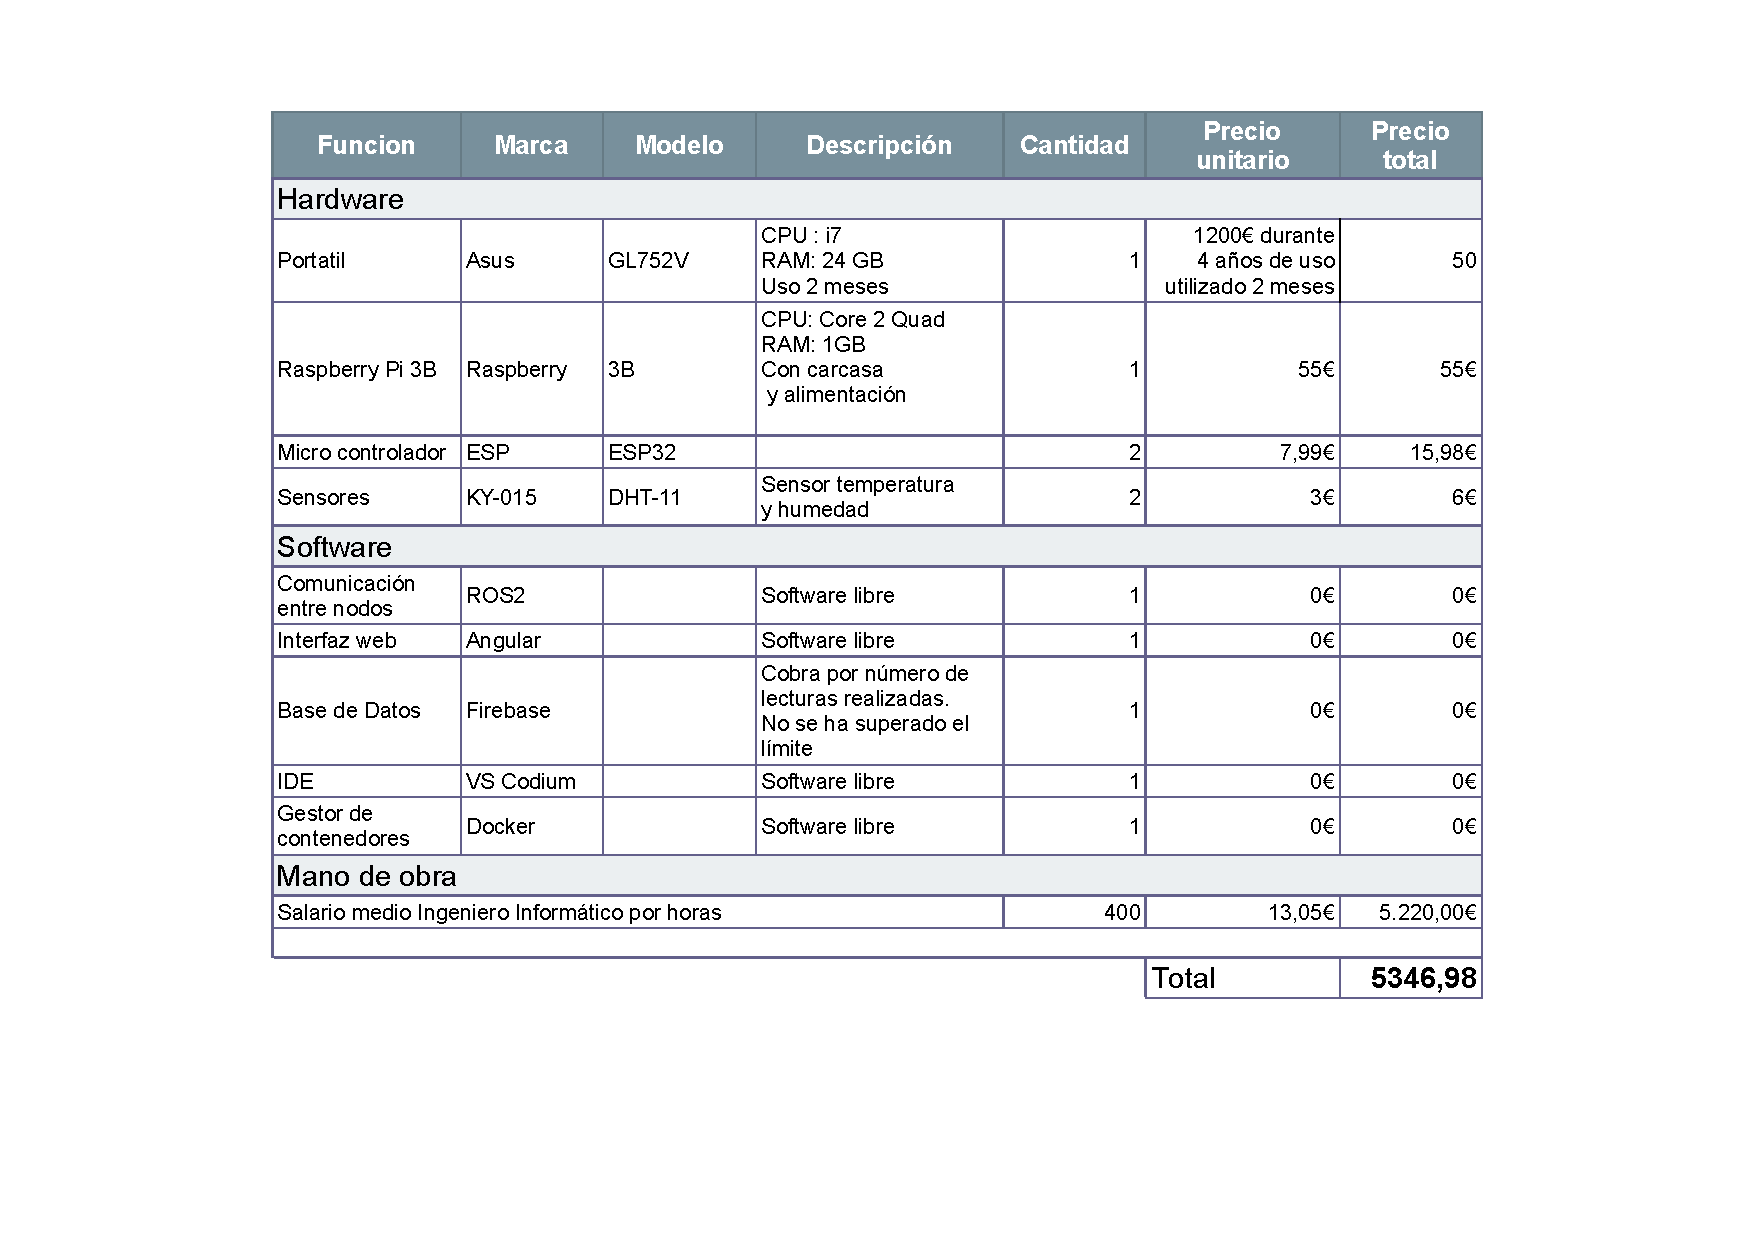
\includegraphics[width=\textwidth]{img/04-Presupuesto.pdf}
    \captionof{figure}{Presupuesto del proyecto}
    \label{fig:presupuesto}
\end{center}

El precio del portátil se ha hecho una estimación de la vida útil, con una media de 4 años, y como se ha utilizado durante 2 meses, el precio correspondiente es ese.

Por lo tanto, el gasto final será de 5346,98€ sumando las diferentes partes. A destacar del gráfico, el presupuesto de ingeniero informático ha sido obtenido de la web Talent.com \cite{salario}, con una media de 13,05€ la hora.

Hay que tener en cuenta que el escenario mayormente será virtual ya que respecto al hardware se van a utilizar diferentes elementos disponibles por casa. Si se tuviese que realizar un presupuesto real sería necesario contactar con diferentes personas con conocimientos relacionados a los sensores del mercado, cableado necesario, elementos para la comunicación, placas a utilizar y estancia de la web en un servidor.

En este caso respecto al hardware se va a utilizar un portátil para el desarrollo y despliegue, una Raspberry Pi 3B con Ubuntu Server y dos placas ESP32 con conectividad wifi junto a sensores DHT-11, cuyo coste se ve reflejado en la tabla anterior \ref{fig:presupuesto}.

\section{Tiempo total empleado}

En la figura \ref{fig:clockify} se pueden visualizar la distribución de horas final recogidas en la aplicación Clockify.

\begin{center}
    \centering
    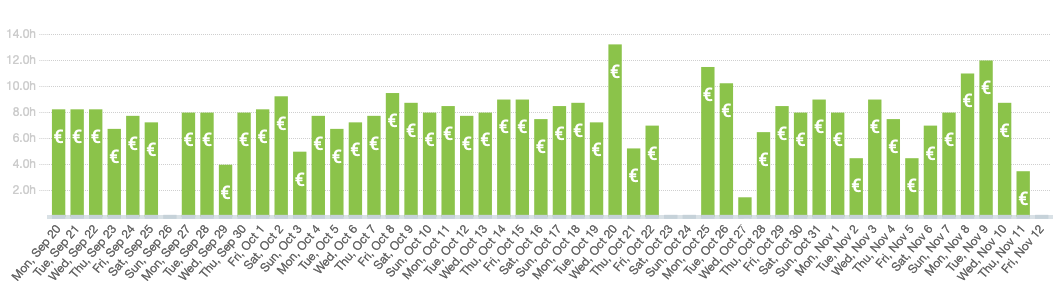
\includegraphics[width=\textwidth]{img/04-diagrama-horas.png}
    \captionof{figure}{Resumen de horas obtenido de Clockify juntando todas las diferentes tareas}
    \label{fig:clockify}
\end{center}

A fecha de la escritura de esta sección, el proyecto ha tomado unas 417h en realizarse, desde la búsqueda de que proyecto a realizar hasta la parte de documentación tras su finalización.

A continuación se adjunta el diagrama de Gantt tras apuntar las tareas realizadas:

\newpage

\begin{center}
    \centering
    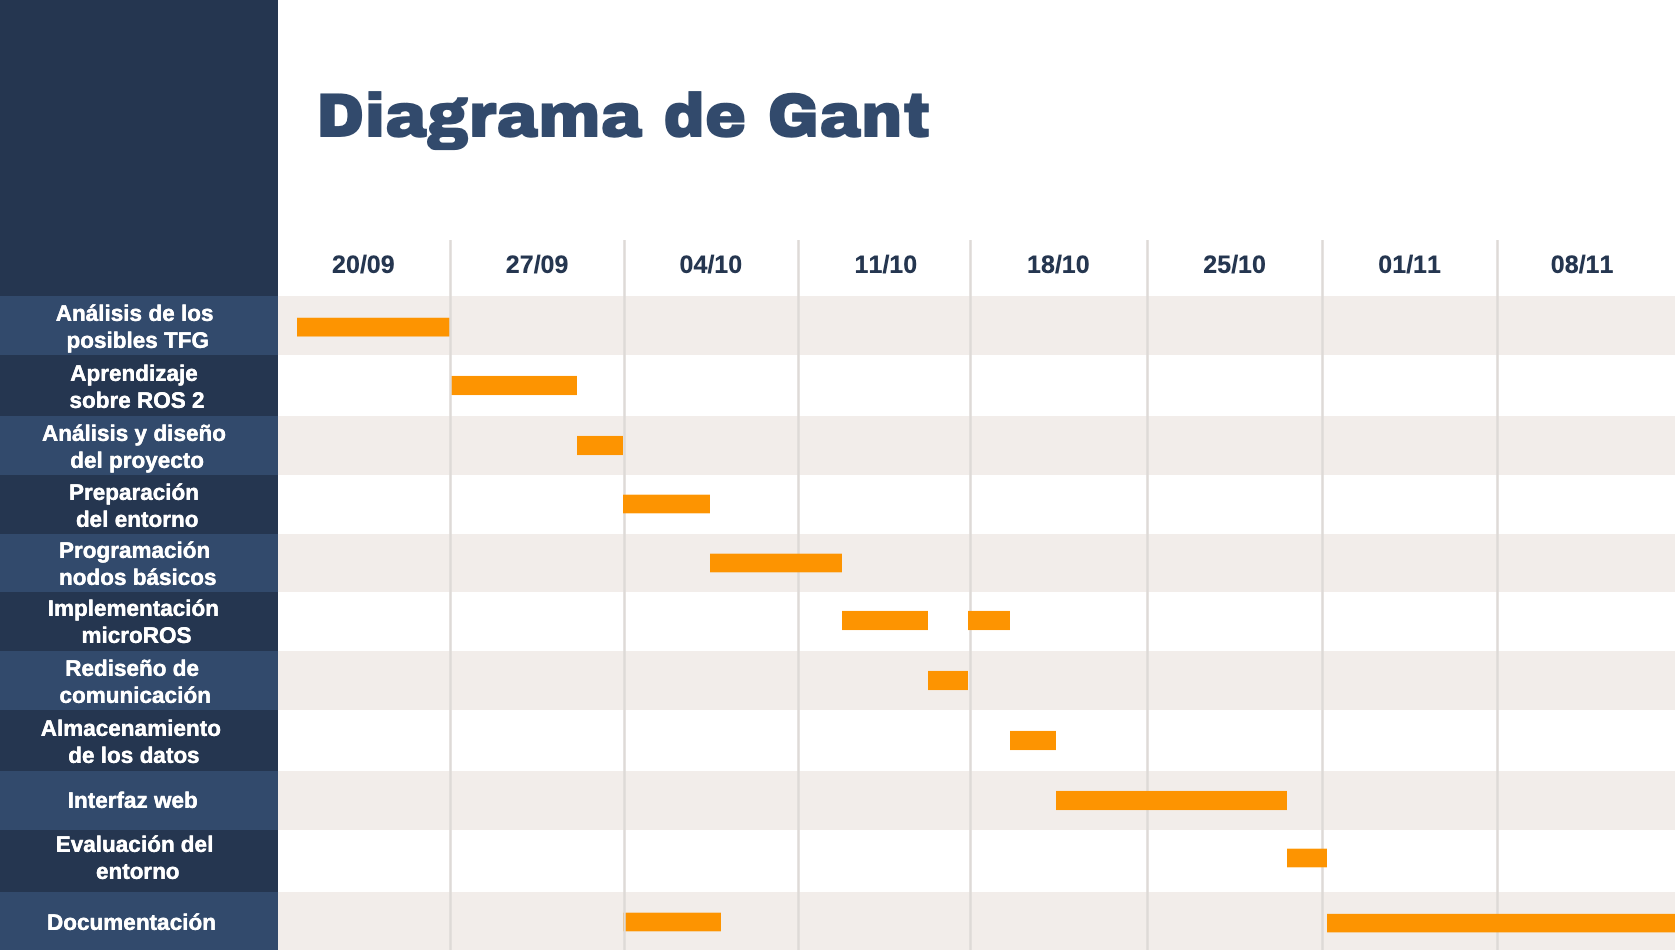
\includegraphics[width=\textwidth]{img/04-Diagrama-Gantt.png}
    \captionof{figure}{Diagrama de Gantt}
    \label{fig:gantt}
\end{center}

A destacar, la tarea del rediseño de comunicación que es la nueva. Esto fue debido a que el tipo de mensaje enviado necesitaba más información de la que se había añadido al principio.